\chapter{Reports Management}
\begin{quote}
\em{Reports that say that something hasn't happened are always interesting to me, because as we know, there are known knowns; there are things we know we know. We also know there are known unknowns; that is to say we know there are some things we do not know. But there are also unknown unknowns - - the ones we don't know we don't know. And if one looks throughout the history of our country and other free countries, it is the latter category that tend to be the difficult ones.}
\begin{flushright}
- Donald H. Rumsfeld ~\cite{rumsfeld}
\end{flushright}
\end{quote}
\section{Requirements}
\subsection{User Requirements}
The following table shows the user requirements for the reports management.
\begin{table}[h]
\centering
\begin{tabular}{p{2cm}p{4.2cm}p{4.2cm}}
\textbf{As a...} & \textbf{I want to...} & \textbf{because...} \\
\hline
Citizen & Report one or more problems with a broken facility & I want it to be fixed \\
Citizen & Track the progress of the reports I've made & I want peace of mind the problem is being resolved \\
Citizen & Be informed the problem has been fixed via email & I might not check the site daily \\
Citizen & Indicate whether or not the problem has fixed once I have been informed & The problem has still not been fixed and I want it so \\
\end{tabular}
\caption{Table of user requirements for the reports management}
\label{tab:reportsrequirements}
\end{table}

\subsection{Software Requirements}
The reports management system needs to be flexible and extendible. This means that any code which is written needs to be as abstract as possible, to take into account reporting for un-envisioned purposes. For example, if a council needs the ability to make reports on things other than facilities, the code should be able to handle the new case with the minimum effort. Ideally, the administrator would create models through the administrator's interface and mark them as ``reportable". This is out of the scope of the project.

\section{Design}
There are already many pieces of viable, useful reports management software. The concern with Taarifa was that plugging in a much larger piece of functionality would be too difficult, even with a well-documented system. For example, when a report is made, it needs to signal the ``find job" part of the website to create a job for the report. Therefore, a stripped down version of a reports management has been created, to show integration with the more interesting problem of job management.

The reports management itself is made from various components, and these are outlined in the sections below.

\subsection{UML Diagram}
The UML diagram shown in Figure~\ref{fig:umlreports} outlines how the objects are viewed in Django, which almost corresponds to their database schema.

\subsubsection{Reportable}
``Reportable" is an abstract class which is designed to be subclassed by things which can be reported. In the use-case of Tandale, an example ``Reportable" would be a part such as a sink tap. More information on how this is used can be found in Section~\ref{sec:facilitiesform}.

\subsubsection{ReportedIssue}
This is also an abstract class which is designed to be subclassed. This is used as the relationship between a report made and the reportable object. Classes which subclass this can add more fields, which are metadata on this relationship.
ReportedIssues are also important, because they are the representation for jobs which workers can apply for. More than one user is able to report the same issue, but only ever one reportedissue for that reportable is in the system at any one time. This is important because it prevents duplication of requests for work.

\subsubsection{Report}
A report is only in the system for the citizen who created it. The description is used on the ReportedIssue view page in order for a worker to have as much information as possible for the task in hand.

\begin{figure}[h]
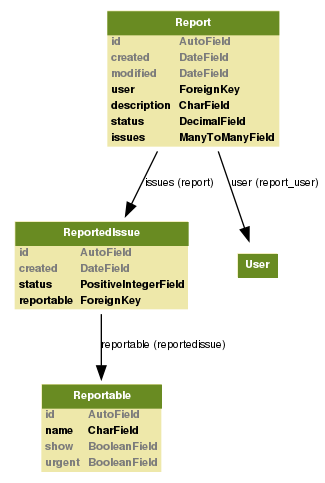
\includegraphics[scale=0.8]{img/reports}
\caption{UML Diagram for the reports management software}
\label{fig:umlreports}
\end{figure}

As the report classes are meant to be overridden, their specific implementation in Taarifa is defined in Chapter~\ref{chap:facilities}.

\section{Implementation}
When the status of a ReportedIssue changes, all users who have reported that issue are emailed notification of the status change. If the status has been changed to ``fixed", they are able to go to the website and indicate whether or not they are satisfied with the change. \\
The Django mail backend sends emails synchronously so if sending to a large number of users, an administrator or worker would have to wait for the emails to send for the page to reload. Thinking that the site had crashed, or something had gone wrong, they may refresh the page. Therefore, it was decided to send the emails asynchronously and Django-celery was intalled.

\subsection{Django-celery~\cite{celery}}
Celery is an asynchronous task queue written in Python; it requires a messaging system which can be any Celery is compatible with. Since it recommends RabbitMQ~\cite{rabbitmq}, and the author has no previous knowledge, RabbitMQ was installed. \\
In order to send messages, the message backend needed to be overwritten. At first, the plugin django-celery-email was installed, but this kept failing with connection refused, so it appeared to not be using the SMTP settings defined in the django settings file. Therefore, django-mailer~\cite{mailer} was installed and configured to work with Celery. \\

\chapter{Facilities}
\label{chap:facilities}
In order for a user to make reports, the classes outlined above must be overridden. There also needs to be a facility manager for an administrator. This section details the main implementation of the reports management.

\section{Requirements}
The table below shows the user requirements for this aspect of the website.

\begin{table}[h]
\centering
\begin{tabular}{p{2cm}p{4.2cm}p{4.2cm}}
\textbf{As a...} & \textbf{I want to...} & \textbf{because...} \\
\hline
Administrator & Create, read, update and delete facilities & The information needs to be in the system and I might want to edit it \\
Worker / Citizen & View facilities on a map & I might want to see where they are \\
\end{tabular}
\caption{Table to show the user requirements for facilities management}
\label{tab:facuser}
\end{table}

\section{Design}
The information for the facilities for this test-case of Taarifa is imported from OpenStreetMap~\cite{openstreetmap}. The data on OpenStreetMap includes many fields, but for the sake of simplicity, a few of those have been excluded. The relevant ones are: location and category. Due to the location aspect of facilities, a part of Django called GeoDjango was enabled.

\subsubsection{GeoDjango}
\label{sec:geodjango}
GeoDjango is built-in with many geospatial functions that can be performed, as well as defining database fields. \\
GeoDjango requires the database provider to be Postgresql, because of the Geometry postgresql enables. For this reason, the database chosen was forcibly Postgresql, but as the author is already comfortable with using this, it was fine. \\
GeoDjango provides a special template to create the database with. Once this had been done, and the appropriate changes made in the Django settings file, Taarifa was geospatially enabled.

\subsubsection{Design}
The following diagram is a UML representation of the facilities management.


\chapter{Design}
The following table shows the user requirements the system needs to implement.

\begin{table}[h]
\centering
\begin{tabular}{p{3.8cm}|p{3.8cm}|p{3.8cm}}
\textbf{As a...} & \textbf{I want to...} & \textbf{because...} \\
\hline
Administrator & Easily change configuration options & What's right for my city may not be the default. \\
\hline
Administrator & Override estimated costs for the jobs associated with the reports & I might know something the system doesn't. \\
\hline
Administrator & Have control over the users who are part of the system & They might abuse the system and I want to block them. \\
\hline
Citizen & Report a problem with a public service & it needs fixing. \\
\hline
Citizen & Check the statuses of the problems I have reported & For peace of mind, I need to know it is being looked at. \\
\hline
Sanitation worker & Find work quickly and easily & I need money. \\
\hline
Sanitation worker & Keep track of the work I have done & I might need the information in the future \\
\hline
Sanitation worker & Get paid & I need money. \\
\end{tabular}
\caption{Table of user requirements}
\label{tab:uses}
\end{table}

\section{MOO}
According to Katkar and Reiley, a secret reserve price is a bad move for the sellers~\cite{ebaypubsec}.
\begin{itemize}
\item The code is badly written in PHP, using a deprecated framework, and MySQL which makes it difficult to maintain and develop. The limitations of MySQL mean it's also bad for Geospatial data. The website therefore has to be ported to a more adaptable, geo-aware system.
\item An administrator has little control over how to configure the system, and therefore needs an administration section.
\item Details of the public facilities are only stored in OpenStreetMap~\cite{openstreetmap} but councils would like their facilities in a database.
\item An administrator in the council might not know the best people to fix the job, and so it should not be the administrator's job to assign people.
\item A user currently makes a very generic report which is not tailor-made to the facility they are reporting. They also have to assign their own urgency to the report, but this can be abused by assigning a high urgency to a non-urgent problem.
\item A user cannot track the reports they have made.
\item A user may make multiple reports on the same problem to artificially prioritise their report.
\item There are no addresses in Tanzania, but the current system asks for an address.
\item The quality of the work performed is not assessed, and a user can only request the status of the report be changed to ``dispute resolution" if they are unhappy with the report.
\end{itemize}
The main aims of this project are:

\begin{itemize}
\item To assess the urgency of a report made.
\item To assign the reports made to people who can fix them.
\item To improve existing report management.
\end{itemize}

\begin{table}[H]
\centering
\begin{tabular}{p{5.7cm}|p{5.7cm}}
\textbf{Problem} & \textbf{Solution} \\
\hline
The code is badly written in PHP and MySQL which makes it difficult to undertake additional development work and is bad for geospatial data.
  & The code has been rewritten with Django using a geospatial Postgresql database. \\
\hline
An administrator has little control over the options.
  & Django's automatic administration abilities have been extended into a fully configurable system. \\
\hline
Details of each facility are not in the database.
  & The facility location and it's category (e.g. toilet or drinking water) are in the database and are easily added, edited and deleted. \\
\hline
Once a report is made, an administrator manually assigns the report to a team; but they may not know the skills nor all the people available to fix the problem.
  & A bidding system where people who can fix problems bid for work. \\
\hline
A user making a report is presented with a generic form which is not tailor-made for the problem they are reporting.
  & An administrator can specify a parts for each category which have a name and a cost (e.g. a tap costs \$3). They can also specify services which can be performed (e.g. drain needs unblocking). This information is used to present a form to the user where they can tick boxes, indicating the problems with the facility. \\
\hline
A user making a report has to specify the urgency of a report, but they can abuse that by setting the urgency artificially high.
  & This option has been removed, and the urgency of the problem is automatically calculated using configuration options set by an administrator. \\
\hline
A user is unable to track the reports they have made; a user could also make multiple reports of the same problem.
  & A login system has been implemented which requires an email address. There are many pros and cons to this decision, which are discussed in Section REFERENCE. \\
There are no addresses in Tanzania.
  & The option to enter an address has been removed and the user clicks on a reportable facility to for a tailor-made form. \\
\hline
The quality of the work performed is not recorded. If a user has a problem with a report marked ``complete", all they can do is request the status of the report be changed to ``dispute resolution", and then it is the responsibility of the administrator to resolve the issue.
  & A user is able to downvote a reported problem if they are not satisfied with the work, and that problem is placed back into the bidding queue.
\end{tabular}
\caption{Table to outline existing problems and the implementation to resolve them}
\label{tab:problems}
\end{table}

\chapter{Background Research}
\section{Mapping Software}
\subsection{MaPit ~\cite{mapit}}
\section{Control Points}
\subsection{B-Splines}
Free-form Deformations are based on linear B-splines, and are a tool used in Computer Graphics to warp the underlying geometry of a model. A mesh is placed across the model, and this is used to compute lattice coordinates for each pixel in the model. Using these lattice coordinates and a function of the tensor product of 1-dimensional B-splines, the new coordinate of the pixels can be calculated.

To apply this idea to Taarifa, each control point would warp the underlying cost of the facilities. The closer a facility is to one of the control points, the higher the inconvenience cost.

An administrator could define the control points, and the boundaries of the region on a map. Although the boundary they define is a polygon, geodjango can return the extent of the polygon, which are coordinates of the bottom left and top right. This method could therefore be used provided those two coordinates (or the alternating two) are known.

This method would work nicely to prevent facilities near lots of control points from being given too high a cost.

The function for 2D linear B-Splines is:

$$u(x, y) = \sum\limits_{m=0}^1\sum\limits_{n=0}^1 B(u)B(v)f\phi_{m+1, n+1}$$

where $B$ is the linear basis function defined as:

$$B_0(s) = 1 - s$$
$$B_1(s) = s$$

$u$ and $v$ are calculated as the displacement of the $x$ and $y$ coordinates from the mesh. $f\phi$ is the function of the control point.

Whilst a modified version of this could work, it will not be implemented. This concept provided the idea of using control points, and therefore was valuable in reaching a final implementation.

\subsection{K-nearest neighbourhood}
This is used in machine learning for classification problems. When a new case is encountered, its classification is determined by how near it is to other points. There are varying implementations of the method. This method, in conjunction with the B-Splines was part of the inspiration.

\chapter{Implementation}
\section{Design}
\section{Configuration}
The first part of implementing the project was to design how an administrator would interact with the system. As Taarifa is envisaged to be a customisable portal with many use cases available, it is important that features can be changed. To this end, Django comes with a highly customisable admin interface which has been used in conjunction with an administrative skin, Grappelli~\cite{grappelli}.

\subsection{Configuration Options}
On the main configuration page, an admistrator is presented with a map, and various fields to fill in. As this project is designed to be as versatile as possible, it can be deployed in various locations with Django's ``site" functionality. This means that each location can have its own configuration, but share all the other data in the system. Therefore, the main configuration page is used on a per site basis.

On this page, a user is presented with a map, where they can draw the boundaries of the region (as a polygon) in which they are working. This is to ensure that only the facilities this particular instance of the site is concerned with are used, which will drastically reduce computation time.

They are also able to place ``control points" on the map. The control points are inspired by Free-Form Deformations from the field of Graphics. The concept is simple: a user defines areas of high economic importance. Facilities around this area will need fixing more quickly than facilities not in the area. Facilities closer to these points will have a higher hidden cost. This is discussed further in Section~\ref{sec:hiddencost}.

For the implementation of this, a piece of javascript was written to allow a user to edit both the bounding box and the control points on the same map. Searching, however, for a nice method of presenting a map to a user in another part of the admin, olwidget~\cite{olwidget} was found. The decision was made to not replace the current work, but then a problem was encountered\footnote{Editing different models on the same map} which olwidget was designed to solve, so olwidget is now used to present maps to the user in the admin section.

The user must draw a bounding box on the map, and also place control points. When placing a control point, a popup box appears, asking them to input the radius of influence that particular control point has. This radius is used in calculations when working out the hidden cost of a job. There is a bug in the olwidget implementation that means once a bounding box has been drawn, the control points radiuses are unable to be edited. This is to do with the way olwidget handles events. This is discussed further in the evaluation section~\ref{sec:thirdparty}.

\subsection{Facilities}
An administrator is able to add a facility to a map by clicking its location. They can then fill in some other fields on a form, and that is saved. Each facility must have a ``Category", which can be edited / added also through the administrative interface. In this instance of Taarifa, each category can have ``Parts" and ``Maintenances". These values are used when constructing the form for a user to make a report. When a new instance of Taarifa is installed elsewhere, these parts and maintenances can be very easily changed by subclassing a class called ``Reportable". The administration screen someone sees is automatically created from all subclasses of this type, which makes Taarifa flexible.

\section{Reporting}
The report management system is a port to Django of the already existing Ushahidi Web. Due to the fact that there are many report management systems, the implementation in Taarifa is as minimalistic as possible, and is implemented solely to show work flow through the system, and to provide proof that the bidding works.

\subsection{Administration}
There is a class called ``Reportable" in the code. Anything subclassing this will be able to be reported, which allows for great flexibility when applying Taarifa to other situations. Anything subclassing this will be automatically handled, so in order to add new situations, a coder has very little work to do. The display to the user uses a piece of code which instantiates a class from a module and a class name. For each subclass of ``Reportable", this code is called, and used to add a display to the Django Admin.

\subsection{Homepage}
The first page a user sees when coming to report a problem is a large map, with markers of all the facilities. The django app, olwidget, has a feature which enables clustering, according to the OpenLayers clustering strategy. To begin with, a user first sees clustered groups of facilities. As they zoom in to where they would like to make a report, the reports which have already been made are displayed. A user can click on a facility and view all the currently open issues with that facility. Because of the way OpenLayers and zooming works, it was initially thought the clustering should be manully turned off when zoomed in far enough. However, the close clustered revealed that there was data repetition in the OpenStreetMap data.

The database for facilities has undergone many changes, so a script was written to read in all the facilities from .osm data. As the facilities are being read, there is now a check in place to ensure that no data points within 12m of each other's centres are added to the database. This not only speeds up the rendering of the map to the user and looks better, but it also ensures that a report is made for the same facility every time.

\section{Bidding}

\subsection{Presentation}
The bids page is sortable by importance\footnote{as determined by a function of the hidden cost and length of time the item has been in the system}, geographical location, and category of item.\footnote{In this implementation - maintenance or service} This is enabled by the third-party app django-filter, which enables subsets of queries to be performed. This has been adapted in order to show a map with all the reported issues.

In the original version of Taarifa, a triaging process was added. The envisaged flow of the report's status was:
\begin{enumerate}
\item Triage: A new report.
\item Verified: An administrator has verified\footnote{Possibly by sending someone to the site, or by recognising a trusted username.} the report.
\item Awaiting Fix: An administrator has forwarded the report to the team responsible for solving the problem.
\item Resolved: The team has fixed the problem, and updated the status accordingly.
\item Dispute Resolution: The person who made the report disagrees the problem has been fixed, and sets the report status to this. An administrator is then responsible for re-forwarding the report.
\end{enumerate} 

This workflow has carried over into the new implementation of Taarifa. Once an administrator has verified the report, the reported issues can be bidded on. Taarifa aims to be a community platform, which means that the administrator should not be the person in charge of allocating the job. This would possibly allow for corruption or nepotism, and the World Bank is keen that does not happen. Therefore the ability for an administrator to assign the job to a particular individual is not present in this implementation. This may change with future versions, and there is an option to allow an administrator to do so in the settings.py file.

Olwidget was used to display maps in the admin interface, but much of the core code was hacked. This is because it was slightly buggy in some places and needed to be patched, but also because it was limiting in the options available.

\subsection{Backend}

The key design factors which were taken into consideration were:
\begin{itemize}
\item Variety of auction.
\item Length of time auction is open for.
\item Which bid to accept.
\end{itemize}

\subsubsection{Which bid to accept}
There are a few factors which determine which bid to accept. Firstly, someone who bids for a job which is lower than the raw material cost of a job will not be accepted. The system is not out to lose people money. Bids lower than the overall hidden cost will be accepted, as the hidden cost is only an estimate.

\subsubsection*{Control Point Calculations}
The control points are in the system with a radius of influence and their location. The influence the control point has over other facilities is proportional to the distance the facility is from the control point. Therefore, the weight must be proportional to the inverse of the distance, which is a linear function. A point much closer to the control point, however, should be much more weighted than a facility at the edge of the influence zone. Furthermore, if the influence of control is short, there will be a large divide between facilities within the zone and facilities outside the zone. In order to smooth out this divide, and to give larger weight to the facilities nearest the control point, the square of the distance will be used instead, and so the control point influence will be $1/d^2$.

\subsubsection{Hidden cost of job}
\label{sec:hiddencost}
The hidden cost is used to decide whether or not to accept higher bids. The hidden cost is a function, as the cost of the facility being broken is increasing by some, unknown, amount per day.

The parameters to take into consideration are:
\begin{itemize}
\item A raw materials cost ($c_i$).
\item Inconvenience cost of part being broken / maintenance being required. $(c_p)$
\item Inconvenience cost of the facility not working. $(c_f)$
\item Inconvenience cost of facility type/category not working. $(c_t)$
\item Inconvenience cost as a result of a function of the distance from the control points. $(c_c)$
\item The length of time since the report was made. $(t)$
\item The number of times the issue has already been reported.
\item The number of reports on the particular facility.
\end{itemize}

The inconvenience cost is either high or low, which corresponds in the system to 10 and 1 respectively. The inconvenience of a part being broken or maintenance required is specific to the type of problem. For example, a dripping tap may have a low inconvenience cost compared to a blocked drain. The inconvenience of the facility itself not working could be that it is the only toilet in a 0.5 mile radius, so may have a high inconvenience cost. The inconvenience cost the category could be that a water tap not working has high inconvenience, but a water fountain\footnote{Not a case covered by this implementation, but both toilets and drinking water are considered to have a high cost} may have low inconvenience. There is additional information, provided by Mark Iliffe, which indicates that a drinking water station and a public toilet have to be more than 2m away from each other, or a broken toilet will cause immense difficulty.

The inconvenience calculated as a distance from control points is useful to ensure that facilities with low inconveniences in the three areas discussed above will receive a higher inconvenience cost, as more people will be affected by the service being out of order. The control points are considered to have uniform weight, but in later releases, this will be changed.

The raw materials cost is a constant which will be added at the end of the calculation taking into consideration the above factors.

The number of times the issue has already been reported and the number of reports on the particular facility are actually an estimate for the true measure of the inconvenience cost of the facility. The database's recorded inconvenience cost to the facility is an administrative estimate, but as more data is collected by the system, the inconvenience costs could be updated from this data. That is out of the scope of this project.

The length of time since a report was made is an important consideration, as it will ensure that jobs with very low priority will still be completed. An artificial cost will be added based on this time. This will not be incorporated into the hidden cost, but will merely be used to bump the importance on the bidding page. \\

To begin designing the function, there are a few edge cases to consider. A facility with high inconvenience costs in all areas on top of a control point should not be weighted with a ludicrously\footnote{The definition of a ludicrous cost is unknown at this time.} high hidden cost.
A facility which is away from the influence of the control points, but itself has a high inconvenience cost should be looked at fairly urgently.

The following table shows the weights of the use cases. As the initial cost is a constant, it has not been included in the table. As the time is a variable, it is also not shown in the table.

\begin{table}
\centering
\begin{tabular}{c|cccc}
\textbf{Use Case} & $c_p$ & $c_f$ & $c_t$ & $c_c$ \\
\hline
High all round & 10 & 10 & 10 & 10 \\
Low all round & 1 & 1 & 1 & 1 \\
Low all round & 1 & 1 & 1 & 1 \\
\end{tabular}
\caption{A table to demonstrate the use cases for the hidden cost function}
\label{tab:hiddencost}
\end{table}

\subsection{Utility Functions}
Work out how much utility they get if they spend all their money on product A by plugging values into the utility function. Do the same for product B. In order to apply a utility function to this situation, we need to assume that the council has a monthly budget (which it does). 

\section{Worker's Rating}
\chapter*{Evaluation}
\section{Testing}
\subsection{DjangoNose}
Nose is a test-runner for Python which speeds up testing and adds different functionality. Django-nose is a wrapper for the test-suite which allows a developer to reuse the test database from the previous run, which means that the speed of testing was greatly improved.
\section*{Third-Party Software}
\subsection*{olwidget}
\label{sec:thirdparty}
\chapter*{Conclusions and Future Work}
\chapter*{Appendix}
\section*{User Guide}